\documentclass[9pt,xcolor={svgnames, x11names},professionalfonts, mathserif]{beamer}
\usepackage{amsmath}
\usepackage{amssymb}
\usepackage{graphicx}
\usepackage{booktabs}  % for top and bottom spacing in table cells
\usepackage{mathpazo}
\usepackage[mathpazo]{flexisym}
\usepackage{breqn}
\usepackage{textcomp}
\usepackage{multirow}
\usepackage{cancel}
\usepackage{array}
%\usepackage{enumerate}
% \usepackage{enumitem} %causes compile error, stack size exceeded?
\usepackage[many]{tcolorbox}
\usepackage{verbatim}
\usepackage{bm}
\usepackage{tkz-linknodes}
\usepackage{gensymb} % for \degree
\usepackage[export]{adjustbox} % for tight borders around photos
\usepackage{pgfmath}


\usepgfmodule{oo}
%\usetikzlibrary{shapes,decorations,shadows,calc}
\usetikzlibrary{shadows,calc,arrows.meta}
% \usetikzlibrary{decorations.shapes}
%\usetikzlibrary{shapes.callouts}
% bloody coils
\usetikzlibrary{decorations.pathmorphing}
\usetikzlibrary{shapes.multipart}



\usepackage{xcolor}
\usepackage{cancel}
\usepackage{bm}
\usepackage{graphicx}
\usepackage[x11names, svgnames]{xcolor} % for colors in handouts, auto loaded in Beamer?
\usepackage{tikz}
\usetikzlibrary{arrows.meta, math, calc, shadows}
\usetikzlibrary{decorations.markings, decorations.fractals, decorations.text} % for chain, etc.
\usetikzlibrary{intersections}
\usepackage{pgfmath}
\usepackage{ifthen}
\usepgfmodule{oo}
\usepgflibrary{shadings}
% \usetikzlibrary{decorations.shapes}
\usepackage[many]{tcolorbox}
\usepackage[absolute,overlay,showboxes]{textpos}
% \usepackage{textpos}
% \textblockorigin{0.0cm}{0.0cm}  %start all at upper left corner
\TPshowboxesfalse

\newcommand\lb{\linebreak}
\newcommand\Ra{\Rightarrow}
\newcommand\cd{\!\cdot\!}
\newcommand\x{\!\times\!}
\newcommand\pars{\par\smallskip}
\newcommand\parm{\par\medskip}
\newcommand\parb{\par\bigskip}
\renewcommand{\deg}{^\circ}

% counter for resuming enumerated list numbers
\newcounter{resumeenumi}
\newcommand{\suspend}{\setcounter{resumeenumi}{\theenumi}}
\newcommand{\resume}{\setcounter{enumi}{\theresumeenumi}}



% https://tex.stackexchange.com/questions/33703/extract-x-y-coordinate-of-an-arbitrary-point-in-tikz
\makeatletter
\providecommand{\gettikzxy}[3]{%
	\tikz@scan@one@point\pgfutil@firstofone#1\relax
	\edef#2{\the\pgf@x}%
	\edef#3{\the\pgf@y}%
}
\makeatother

\makeatletter
\newcommand{\verbatimfont}[1]{\def\verbatim@font{#1}}%
\makeatother

%%%%%%%%%%%%%%%%%%%%%%%%%%%%%%%%%%%%%%%%%%%%%%%%%%%%%%%%%%%%%%%%%%%%%%%%%%%%%%%%


\newcommand{\tb}[4][0.8]{
	\begin{textblock*}{#1}(#2, #3)
		% \raggedright
		#4
	\end{textblock*}
}

\newtcolorbox{statsbox}[2][] { 
  colback=white,
  colbacktitle=structure,
  colframe=structure,
  coltitle=white,  
  top=0.25cm,
	bottom=0.125cm,
	left=0mm,
	right=0mm,
  % fonttitle=\itshape\rmfamily,
  halign=flush left, 
  enhanced,
  drop fuzzy shadow,
  attach boxed title to top left={xshift=3.5mm, yshift=-2mm},
  title={#2}, #1}
\newtcolorbox{redbox}{colback=white, colframe=structure, enhanced, drop fuzzy shadow}
\newtcolorbox{titledbox}[1]{colback=white,colframe=structure,title={#1}}
\newtcbox{\tcb}[1][]{colback=white,boxsep=0pt,top=5pt,bottom=5pt,left=5pt,
		right=5pt, colframe=structure,  enhanced, drop fuzzy shadow, #1}
% tcb title
\newtcbox{\tcbt}[2][]{colback=white,boxsep=0pt,top=5pt,bottom=5pt,left=5pt,
		right=5pt, colframe=structure, enhanced, drop fuzzy shadow,  title={#2}, #1}
% tcb left title
\newtcbox{\tcbtl}[2][]{ colback=white,
  colbacktitle=structure,
  colframe=structure,
  coltitle=white,  
  top=0.25cm,
	bottom=0.125cm,
	left=0mm,
	right=0mm,
  % fonttitle=\bfseries,
  halign=flush left, 
  enhanced,
  drop fuzzy shadow,
  attach boxed title to top left={xshift=3.5mm, yshift=-2mm}, 
	title={#2}, #1}

\newtcbtheorem{myexam}{Example}%
{
	enhanced,
	colback=white,
	colframe=structure,
	% fonttitle=\bfseries,
	fonttitle=\itshape\rmfamily,
	drop fuzzy shadow,
	%description font=\mdseries\itshape,
	attach boxed title to top left={yshift=-2mm, xshift=5mm},
	colbacktitle=structure
	}{exam}% then \pageref{exer:theoexample} references the theo

% \newcommand{\myexample}[2][red]{
% 	% \tcb\tcbset{theostyle/.style={colframe=red,colbacktitle=yellow}}
% 	\begin{myexam}{}{}
% 		#2
% 	\end{myexam}
% 	% \tcbset{colframe=structure,colbacktitle=structure}
% }

\newtcbtheorem{myexer}{Exercise}%
{
	enhanced,
	colback=white,
	colframe=structure,
	% fonttitle=\bfseries,
	drop fuzzy shadow,
	fonttitle=\itshape\rmfamily,
	% description font=\mdseries\itshape,
	attach boxed title to top left={yshift=-2mm, xshift=5mm},
	colbacktitle=structure
	}{exer}



\newcommand{\mini}[2][0.8]{
	\begin{minipage}[c]{#1\columnwidth}
		\raggedright
		#2
	\end{minipage}
}
\newcommand{\minit}[2][0.8]{
	\begin{minipage}[t]{#1\columnwidth}
		% \raggedright
		#2
	\end{minipage}
}

% centered minipage with text \raggedright
%\cmini[width]{content}
\newcommand{\cmini}[2][0.8]{
	\begin{center}
		\begin{minipage}{#1\columnwidth}
			\raggedright
			#2
		\end{minipage}
	\end{center}
}



\newcommand{\fig}[2][1]{% scaled graphic
	\includegraphics[scale=#1]{#2}
}

% centred framed colored box black border
%\cbox[width]{content}
\newcommand{\cbox}[2][1]{% framed centered color box
	\setlength\fboxsep{5mm}
	\setlength\fboxrule{.2 mm}
	\begin{center}
		\fcolorbox{black}{white}{
			\vspace{-0.5cm}
			\begin{minipage}{#1\columnwidth}
				\raggedright
				#2
			\end{minipage}
		}
	\end{center}
	\setlength\fboxsep{0cm}
}

\newcommand{\cfig}[2][1]{% centred, scaled graphic
	\begin{center}
		\includegraphics[scale=#1]{#2}
	\end{center}
}






 \definecolor{saitPurple}{RGB}{112,40,119}
 \definecolor{statsMaroon}{rgb}{0.55, 0, 0}
 \definecolor{saitMaroon}{rgb}{0.55, 0, 0}
 \definecolor{statsRed}{RGB}{224,38,37}
 \definecolor{saitRed}{RGB}{224,38,37}
 \definecolor{saitBlue}{rgb}{0, 0.59, 0.85}
 \definecolor{statsBlue}{rgb}{0, 0.59, 0.85}
 \definecolor{statsDeepBlue}{RGB}{0, 99, 167}
 \definecolor{saitDeepBlue}{RGB}{0, 99, 167}
 \definecolor{saitDeepBlue}{RGB}{0, 99, 167}
 \definecolor{LightGrey}{RGB}{200,200,200}
%  \definecolor{boxBG}{RGB}{236, 227, 227}
%  \definecolor{boxBG}{RGB}{242, 233, 223}
% \begin{comment}
% Shadings are useful to give the illusion of 3D in examples and exercises presented to engineering technology students.
% Vertical and horizontal shadings of rectangles are fairly straightforward to produce with the shading library included in
% a recent build of Tikz.
% Rotation of shaded squares is also intuitive, but rotation of a shaded rectangle appears to be both a function of the specified
% rotation angle and the length to width ratio of the rectangle. This makes aligning the shading of a rotated rectangle's
% fill with the stroke of a rotated rectangle a bit of an inelegant trial-and-error exercise (for me, at any rate).
%
%
% \end{comment}

%http://tex.stackexchange.com/questions/33703/extract-x-y-coordinate-of-an-arbitrary-point-in-tikz
\makeatletter
\providecommand{\gettikzxy}[3]{%
	\tikz@scan@one@point\pgfutil@firstofone#1\relax
	\edef#2{\the\pgf@x}%
	\edef#3{\the\pgf@y}%
}
\makeatother


%%%%%%%%%%%%%%%%%%%%%%%%%%%%%%%% A CLASS FOR ROTATED RECTANGLES WITH A SHADED FILL %%%%%%%%%%%%%%%%%%%%%%%%%%%%%%%%%%%%%%%%


		\pgfooclass{rrect}{
			\method rrect(#1,#2,#3,#4,#5,#6,#7,#8,#9) { % The constructor; everything is done in here
			\def\pt2cm{28.4556}
			\gettikzxy{(#1)}{\spx}{\spy}
			\gettikzxy{(#2)}{\epx}{\epy}
				\def\outercolor{#3} \def\innercolor{#4}
				\def\stroke{#5} \def\HI{#6} \def\RADII{#7} \def\extend{#8} \def\LINEWIDTH{#9}
				\pgfmathparse{divide(\spx,\pt2cm)} \let\STARTX\pgfmathresult
				\pgfmathparse{divide(\spy,\pt2cm)} \let\STARTY\pgfmathresult
				\pgfmathparse{divide(\epy,\pt2cm)} \let\ENDY\pgfmathresult
				\pgfmathparse{divide(\epx,\pt2cm)} \let\ENDX\pgfmathresult
				\pgfmathparse{\ENDX-\STARTX} \let\deltaX\pgfmathresult
				\pgfmathparse{\ENDY-\STARTY} \let\deltaY\pgfmathresult
				\ifthenelse{\equal{\deltaX}{0.0}}
				{	% vertical rod is a special case; otherwise atan gets a div by 0 error
					\pgfmathparse{\ENDY>\STARTY} \let\ccw\pgfmathresult
					\ifthenelse{\equal{\ccw}{1}}{%
						\def\rot{90}}
					{\def\rot{-90}}}
			{	% not vertical
				\pgfmathparse{\STARTX<\ENDX} \let\iseast\pgfmathresult
				\ifthenelse{\equal{\iseast}{1}}{%
					\pgfmathparse{atan(\deltaY/\deltaX)} \let\rot\pgfmathresult
				} % end is east
				{
					\pgfmathparse{180+atan(\deltaY/\deltaX)} \let\rot\pgfmathresult
				} % end !east
				}
				%shading boundaries work for vertical and horizontal but otherwise ``spills'' outside it supposed boundaries,
				%particularly at multiples of 45deg
				%make some adjustments from a max at 45 to nothing at 0 or 90
				\pgfmathparse{abs(\deltaY)} \let\absdeltaY\pgfmathresult
				\pgfmathparse{abs(\deltaX)} \let\absdeltaX\pgfmathresult
				%\def\shadeangle{-42}
				\ifthenelse{\equal{\deltaX}{0.0}}
				{\def\shadeangle{0.0}}
				{\pgfmathparse{\absdeltaY > \absdeltaX} \let\foo\pgfmathresult
					\ifthenelse{\equal{\foo}{1}}
					{\pgfmathparse{90-atan(\absdeltaY/\absdeltaX)} \let\shadeangle\pgfmathresult}
					{\pgfmathparse{atan(\absdeltaY/\absdeltaX)} \let\shadeangle\pgfmathresult}
				}
				\pgfmathparse{tan(\shadeangle)} \let\fudge\pgfmathresult
				\pgfmathparse{veclen(\deltaX,\deltaY)} \let\len\pgfmathresult
				\pgfmathparse{max(\HI,\len+2*\extend)} \let\shadeboxside\pgfmathresult
				\pgfmathparse{50-25/\shadeboxside*\HI+8*\HI*\fudge/\shadeboxside} \let\mybot\pgfmathresult
				\pgfmathparse{50+25/\shadeboxside*\HI-8*\HI*\fudge/\shadeboxside} \let\mytop\pgfmathresult
				\pgfdeclareverticalshading{myshade}{100bp}{%
					color(0bp)=(\outercolor);
					color(\mybot bp)=(\outercolor);
					color(50 bp)=(\innercolor);
					color(\mytop bp)=(\outercolor);
					color(100bp)=(\outercolor)}
				\tikzset{shading=myshade}
				\begin{scope}	[rotate around = {\rot:(\STARTX, \STARTY )}]
					\begin{scope}
						\draw[clip, rounded corners = 0.5*\scale*\RADII cm] (\STARTX-\extend/2,\STARTY-\HI/2) rectangle +(\len+2*\extend/2,\HI);
						\shade[ shading angle=\rot] (\STARTX-\extend,\STARTY-\shadeboxside/2) rectangle +(\shadeboxside, \shadeboxside);
					\end{scope} %end clipping
					\draw[rounded corners=0.5*\scale*\RADII cm, \stroke, line width=\LINEWIDTH mm] (\STARTX-\extend/2,\STARTY-\HI/2) rectangle +(\len+2*\extend/2,\HI);
				\end{scope}
				} % end of constructor
				} % end of rrect class

		% \pgfooclass{rr}{
		% 	\method rr(#1,#2,#3,#4,#5) { % The constructor; everything is done in here
		% 		% Here I can get named x and y coordinates
		% 		\def\phil{#3} \def\stroke{#4} \def\line{#5}
		% 		\gettikzxy{(#1)}{\spx}{\spy}
		% 		\gettikzxy{(#2)}{\epx}{\epy}
		% 		% I'd like named points to work with
		% 		\coordinate (Start) at (\spx, \spy);
		% 		\coordinate (End) at (\epx, \epy);
		% 		% Find the length between start and end. Then the angle between x axis and Diff will be the rotation to apply.
		% 		\coordinate (Diff) at ($ (End)-(Start) $);
		% 		\gettikzxy{(Diff)}{\dx}{\dy}
		% 		\pgfmathparse{veclen(\dx, \dy)} \pgfmathresult
		% 		\let\length\pgfmathresult
		% 		\pgfmathparse{\dx==0}%
		% 		% \ifnum low-level TeX for integers
		% 		\ifnum\pgfmathresult=1 % \dx == 0
		% 			\pgfmathsetmacro{\rot}{\dy > 0 ? 90 : -90}
		% 		\else% \dx != 0
		% 			\pgfmathsetmacro{\rot}{\dx > 0 ? atan(\dy / \dx) : 180 + atan(\dy / \dx)}
		% 		\fi
		% 		\begin{scope}	[rotate around ={\rot:(Start)}]
		% 			% \filldraw[ultra thick, fill=\phil, draw=\stroke] ($ (Start)+(0,\HI) $) arc(90:270:\HI) -- +(\length pt, 0) arc(-90:90:\HI) -- cycle;
		% 			\filldraw[rounded corners=\scale*\radii cm, line width=\line mm, fill=\phil, draw=\stroke] (\spx-\extend cm,\spy-\hi cm) rectangle +(2*\extend cm + \length pt, 2*\hi cm);
		% 		\end{scope}
		% 	}
		% }

		
		% \pgfooclass{beam}{
		% 	\method beam(#1,#2,#3,#4,#5) { % The constructor; everything is done in here
		% 		% Here I can get named x and y coordinates
		% 		\def\phil{#3} \def\stroke{#4} \def\line{#5}
		% 		\gettikzxy{(#1)}{\spx}{\spy}
		% 		\gettikzxy{(#2)}{\epx}{\epy}
		% 		% I'd like named points to work with
		% 		\coordinate (Start) at (\spx, \spy);
		% 		\coordinate (End) at (\epx, \epy);
		% 		% Find the length between start and end. Then the angle between x axis and Diff will be the rotation to apply.
		% 		\coordinate (Diff) at ($ (End)-(Start) $);
		% 		\gettikzxy{(Diff)}{\dx}{\dy}
		% 		\pgfmathparse{veclen(\dx, \dy)} \pgfmathresult
		% 		\let\length\pgfmathresult
		% 		\pgfmathparse{\dx==0}%
		% 		% \ifnum low-level TeX for integers
		% 		\ifnum\pgfmathresult=1 % \dx == 0
		% 			\pgfmathsetmacro{\rot}{\dy > 0 ? 90 : -90}
		% 		\else% \dx != 0
		% 			\pgfmathsetmacro{\rot}{\dx > 0 ? atan(\dy / \dx) : 180 + atan(\dy / \dx)}
		% 		\fi
		% 		\begin{scope}	[rotate around = {\rot:(\spx, \spy )}]
		% 			\fill[\phil] (\spx-\extend cm,\spy-\HI cm) rectangle +( 2*\extend cm + \length pt, 2*\HI cm );
		% 			\draw[draw=\stroke, line width=\line mm] (\spx-\extend cm,\spy-\HI cm) -- +(2*\extend cm + \length pt, 0);
		% 			\draw[draw=\stroke, line width=\line mm] (\spx-\extend cm,\spy+\HI cm) -- +(2*\extend cm + \length pt, 0);
		% 		\end{scope}
		% 	}
		% }

		\pgfooclass{beam}{
			\method beam(#1,#2,#3,#4,#5,#6,#7) { % The constructor; everything is done in here
				% Here I can get named x and y coordinates
				\def\phil{#3} \def\stroke{#4} \def\HI{#5} \def\extend{#6} \def\LINEWIDTH{#7}
				\gettikzxy{(#1)}{\spx}{\spy}
				\gettikzxy{(#2)}{\epx}{\epy}
				% I'd like named points to work with
				\coordinate (Start) at (\spx, \spy);
				\coordinate (End) at (\epx, \epy);
				% Find the length between start and end. Then the angle between x axis and Diff will be the rotation to apply.
				\coordinate (Diff) at ($ (End)-(Start) $);
				\gettikzxy{(Diff)}{\dx}{\dy}
				\pgfmathparse{veclen(\dx, \dy)} \pgfmathresult
				\let\length\pgfmathresult
				\pgfmathparse{\dx==0}%
				% \ifnum low-level TeX for integers
				\ifnum\pgfmathresult=1 % \dx == 0
					\pgfmathsetmacro{\rot}{\dy > 0 ? 90 : -90}
				\else% \dx != 0
					\pgfmathsetmacro{\rot}{\dx > 0 ? atan(\dy / \dx) : 180 + atan(\dy / \dx)}
				\fi
				\begin{scope}	[rotate around = {\rot:(\spx, \spy )}]
					\fill[\phil] (\spx-\extend cm,\spy-\HI cm) rectangle +( 2*\extend cm + \length pt, 2*\HI cm );
					\draw[draw=\stroke, line width=\LINEWIDTH mm] (\spx-\extend cm,\spy-\HI cm) -- +(2*\extend cm + \length pt, 0);
					\draw[draw=\stroke, line width=\LINEWIDTH mm] (\spx-\extend cm,\spy+\HI cm) -- +(2*\extend cm + \length pt, 0);
				\end{scope}
			}
		}

		% \pgfooclass{bottomChord}{
		% 	\method beam(#1,#2,#3,#4,#5) { % The constructor; everything is done in here
		% 		% Here I can get named x and y coordinates
		% 		\def\phil{#3} \def\stroke{#4} \def\line{#5}
		% 		\gettikzxy{(#1)}{\spx}{\spy}
		% 		\gettikzxy{(#2)}{\epx}{\epy}
		% 		% I'd like named points to work with
		% 		\coordinate (Start) at (\spx, \spy);
		% 		\coordinate (End) at (\epx, \epy);
		% 		% Find the length between start and end. Then the angle between x axis and Diff will be the rotation to apply.
		% 		\coordinate (Diff) at ($ (End)-(Start) $);
		% 		\gettikzxy{(Diff)}{\dx}{\dy}
		% 		\pgfmathparse{veclen(\dx, \dy)} \pgfmathresult
		% 		\let\length\pgfmathresult
		% 		\pgfmathparse{\dx==0}%
		% 		% \ifnum low-level TeX for integers
		% 		\ifnum\pgfmathresult=1 % \dx == 0
		% 			\pgfmathsetmacro{\rot}{\dy > 0 ? 90 : -90}
		% 		\else% \dx != 0
		% 			\pgfmathsetmacro{\rot}{\dx > 0 ? atan(\dy / \dx) : 180 + atan(\dy / \dx)}
		% 		\fi
		% 		\begin{scope}	[rotate around = {\rot:(\spx, \spy )}]
		% 			% \fill[\phil] (\spx-\extend cm,\spy-\HI cm) rectangle +(2*\extend cm + \length pt, 2*\HI cm);
		% 			% \draw[draw=\stroke, line width=\line mm] (\spx-\extend cm,\spy-\HI cm) -- +(2*\extend cm + \length pt, 0);
		%
		% 			\draw[draw=\stroke, line width=\line mm] (\spx-\extend cm,\spy+\HI cm) -- +(2*\extend cm + \length pt, 0);
		% 			\draw[draw=\stroke, line width=\line mm] (\spx-\extend cm,\spy+\HI cm) -- +(2*\extend cm + \length pt, 0);
		% 		\end{scope}
		% 	}
		% }

% !TEX root = ../Beamer/statikz/statikz.tex

% \Channel[rotate=0]{coordinate}{draw}{fill}{scale}{lineWidth}
\newcommand{\Channel}[6][0]{
	\def\rotate{#1};
	\def\mid{#2}
	\def\lfill{#3}
	\def\lstroke{#4}
	\def\scale{#5};
	\def\lineWidth{#6};

	\begin{scope}[rounded corners=1pt, scale=\scale, rotate=\rotate]
		\filldraw[draw=\lstroke, fill=\lfill, line width=\lineWidth pt] ($(\mid) + (0,-3) $) -- ++(1.7,0) arc(0:85:0.25) -- ($ (\mid)+(0.4,-2.6) $) -- ($ (\mid)+(0.4,2.6) $) -- +(8.13:1.097)arc(-81.87:0:0.25) -- ($ (\mid)+(0,3) $)  -- cycle;
	\end{scope}
}

% !TEX root = ../Beamer/statikz/statikz.tex

%\DLOne[rotate]{tl}{tr}{b}{fill}{draw}{spaces}{scale}{lineWidth}
\newcommand{\DLOne}[9][0]{
	\def\rotate{#1}
	\def\tl{#2}
	\def\tr{#3}
	\def\b{#4}
	\def\lfill{#5}
	\def\ldraw{#6}
	\def\spaces{#7}
	\def\lscale{#8}
	\def\llinewidth{#9}

	\def\tocm{0.0351459804}
	\providecommand\tiplength{2.5pt}

	\gettikzxy{(\tl)}{\tlx}{\tly};
	\gettikzxy{(\tr)}{\trx}{\try};
	\gettikzxy{(\b)}{\bx}{\by};

	\pgfmathparse{\trx-\tlx} \let\dx\pgfmathresult
	\pgfmathparse{\try-\tly} \let\dy\pgfmathresult
	\pgfmathparse{round(\tocm*\dx*100)/100} \let\dxcm\pgfmathresult
	\pgfmathparse{round(\tocm*\dy*100)/100} \let\dycm\pgfmathresult

	\coordinate (midBase) at (\tlx/2+\trx/2, \by);

	\gettikzxy{(midBase)}{\mx}{\my}
	\pgfmathparse{round(\tocm*\mx*100)/100} \let\mxcm\pgfmathresult
	\pgfmathparse{round(\tocm*\my*100)/100} \let\mycm\pgfmathresult


	\pgfmathparse{\dxcm/\spaces} \let\xspacing\pgfmathresult
	\pgfmathparse{\dycm/\spaces} \let\yspacing\pgfmathresult
	\pgfmathparse{\spaces-1} \let\numarrows\pgfmathresult

	\begin{scope}[scale=\lscale, rotate around ={\rotate:(midBase)}, line cap = round, line join = round, line width = \llinewidth mm]
		\fill[\lfill] (\tlx, \tly) -- (\trx, \try) -- (\trx, \by) -- (\tlx, \by);
		\draw[\ldraw!50, thin] (\tlx, \by) -- (\trx, \by);
		% \draw (\mxcm,\mycm) circle (2pt) node[below] {\mxcm, \mx};
		% \draw (midBase) circle (2pt)node[above] {\my};
		% \draw (\bx, \by) circle (2pt) node[above] {\by};

		\pgfmathparse{abs(\try - \by)} \let\ryy\pgfmathresult
		\pgfmathparse{abs(\tly - \by)} \let\lyy\pgfmathresult

		\pgfmathparse{\lyy>\tiplength && \ryy>\tiplength}
		\ifnum\pgfmathresult=1
			\draw[\ldraw, {Straight Barb[length=\tiplength]}-{Straight Barb[length=\tiplength]},line width=\llinewidth] (\tlx,\by) -- (\tlx, \tly) -- (\trx,\try) -- (\trx,\by);
		\fi
		\pgfmathparse{\lyy<\tiplength && \lyy>\tiplength/4 && \ryy>\tiplength}
		\ifnum\pgfmathresult=1
			\draw[\ldraw, {Straight Barb[length=\lyy]}-{Straight Barb[length=\tiplength]},line width=\llinewidth] (\tlx,\by) -- (\tlx, \tly) -- (\trx,\try) -- (\trx,\by);
		\fi
		\pgfmathparse{\lyy<=\tiplength/4 && \ryy>\tiplength}
		\ifnum\pgfmathresult=1
			\draw[\ldraw, -{Straight Barb[length=\tiplength]},line width=\llinewidth] (\tlx,\by) -- (\tlx, \tly) -- (\trx,\try) -- (\trx,\by);
		\fi
		\pgfmathparse{\ryy<\tiplength && \ryy>\tiplength/4 && \lyy>\tiplength}
		\ifnum\pgfmathresult=1
			\draw[\ldraw, {Straight Barb[length=\tiplength]}-{Straight Barb[length=\ryy]},line width=\llinewidth] (\tlx,\by) -- (\tlx, \tly) -- (\trx,\try) -- (\trx,\by);
		\fi
		\pgfmathparse{\ryy<=\tiplength/4 && \lyy>\tiplength}
		\ifnum\pgfmathresult=1
			\draw[\ldraw, {Straight Barb[length=\tiplength]}-,line width=\llinewidth] (\tlx,\by) -- (\tlx, \tly) -- (\trx,\try) -- (\trx,\by);
		\fi

	%
		\begin{scope}
			\clip (\tlx,\tly) -- (\trx, \try) -- (\trx,\by) -- (\tlx,\by) ;
			\foreach \i in {1,...,\numarrows}
			\def\x{\i*\xspacing}
			\def\y{\i*\yspacing}
			\draw[\ldraw, -{Straight Barb[length=\tiplength]}, line width = \llinewidth pt] ($ (\tlx,\tly)+(\x,\y) $) -- ($ (\tlx,\by)+(\x,0) $);
		\end{scope}
	\end{scope}
	% \draw (midBase) circle (3pt)node[below]{\yspacing};
}

% !TEX root = ../Beamer/02ForceVectors/02ForceVectors.tex


\newcommand{\EyeBolt}[6][0]{
	\def\lrotate{#1};
	\def\lpin{#2}
	\def\lfill{#3}
	\def\ldraw{#4}
	\def\lscale{#5}
	\def\lwidth{#6}
	%\def\h{1.5}
	\def\r{0.3}
	\begin{scope}[scale=\lscale, rotate=\lrotate]
		\filldraw[draw=\ldraw, fill=\lfill, line width=\lwidth pt] ($(\lpin) + (-0.7,-1.25)$) arc(180:90:.2) -- ++(0.05,0)arc(-90:0:0.2) -- ++(0.05,0.65)arc(225:-45:0.28284)-- ++(0.05,-.65)arc(180:270:.2)-- ++(0.05,0)arc(90:0:0.2) -- cycle;
		\fill[outer color=\lfill, inner color=black, line width = 0] (\lpin) circle (2.25mm);
		\filldraw[fill=white, draw=\ldraw, line width = \lwidth pt] (\lpin) circle (1.25mm);

		\begin{scope}[even odd rule]
			\fill[\lfill] (\lpin) circle (2.5mm)
			(\lpin) circle (2.125mm);
		\end{scope}

		\filldraw[rounded corners=\lscale pt, draw=\ldraw, fill=\lfill, line width=\lwidth pt] ($ (\lpin) - (1,1.5) $) rectangle +(2,0.25);
	\end{scope}
}

% !TEX root = ../../Beamer/statikz/statikz.tex


\newcommand{\EyeConnection}[6][0]{
	\def\lrotate{#1};
	\def\lpin{#2}
	\def\lfill{#3}
	\def\ldraw{#4}
	\def\lscale{#5}
	\def\lwidth{#6}
	\def\h{1}
	\def\r{0.3}
	\begin{scope}[scale=\lscale, rotate=\lrotate]
		\filldraw[draw=\ldraw, fill=\lfill, line width=\lwidth pt] ($(\lpin) + (0.201*\h+1.0353*\r ,-0.75*\h)$) -- ++(105: 0.77646*\h+0.26795*\r) arc (15:165:\r) -- ++(-105:0.77646*\h+0.26795*\r) -- cycle;

		\fill[outer color=\lfill, middle color=red, inner color=black, line width = \lwidth pt] (\lpin) circle (2.5mm);
		\filldraw[fill=white, draw=\ldraw, line width = \lwidth pt] (\lpin) circle (1.25mm);

		\filldraw[rounded corners=\lscale pt, draw=\ldraw, fill=\lfill, line width=\lwidth pt] ($ (\lpin) - (1,1) $) rectangle +(2,0.25);
	\end{scope}
}

\input{../../Includes/PinnedConnection.tex}
% !TEX root = ../Beamer/statikz/statikz.tex

% \Pulley[rotation]{A}{wheel color}{support color}{scale}{line width}
\newcommand{\Pulley}[6][0]{
	\def\lrotate{#1};
	\def\lpin{#2}
	\def\lfill{#3}
	\def\ldraw{#4}
	\def\lscale{#5}
	\def\lwidth{#6}
	\def\h{1}
	\def\r{0.35}
	\def\rr{0.675}
	\begin{scope}[scale=\lscale, rotate=\lrotate]

		\filldraw[draw=\ldraw, fill=\lfill, line width=\lwidth mm] (\lpin) circle (\h*\rr cm);

		\filldraw[draw=\ldraw, fill=\lfill!70!black, line width=\lwidth mm] (\lpin) circle (\h*\rr*0.75 cm);

		\filldraw[draw=\ldraw, fill=\lfill, line width=\lwidth mm] ($(\lpin) + (0.201*\h+1.0353*\r ,-0.75*\h)$) -- ++(105: 0.77646*\h+0.26795*\r) arc (15:165:\r) -- ++(-105:0.77646*\h+0.26795*\r) -- cycle;

		\shadedraw[ball color=\lfill, draw=\ldraw, line width = \lwidth mm] (\lpin) circle (2*\h*\rr mm);

		\filldraw[rounded corners=\lscale pt, draw=\ldraw, fill=\lfill, line width=\lwidth mm] ($ (\lpin) - (1,1) $) rectangle +(2,0.25);
	\end{scope}
}

% !TEX root = ../Beamer/statikz/statikz.tex

% \Ring{A}{outer color}{inner color}{outer radius}{inner radius}{line width}
\newcommand{\Ring}[6]{
	\def\lpin{#1}
	\def\lfill{#2}
	\def\ldraw{#3}
	\def\outerr{#4}
	\def\innerr{#5}
	\def\lwidth{#6}

	\begin{scope}

		\makeatletter
		\providecommand{\gettikzxy}[3]{%
			\tikz@scan@one@point\pgfutil@firstofone#1\relax
			\edef#2{\the\pgf@x}%
			\edef#3{\the\pgf@y}%
		}
		\makeatother

		\gettikzxy{(\lpin)}{\cx}{\cy}
		\pgfdeclareradialshading{ring}{\pgfpoint{0cm}{0cm}}
		{
			color(0cm)=(black);
			color(0.5cm)=(\lfill);
			color(.65cm)=(\ldraw);
			color(1cm)=(\lfill)
		}
		% \pgfuseshading{ring}



	\end{scope}


\begin{scope}[even odd rule]
	% \draw (\lpin) circle (\innerr);
	\filldraw[shading=ring, fill=\lfill, draw=\ldraw, line width=\lwidth] (\lpin) circle (\outerr cm)
		(\lpin) circle (\innerr);
		\draw[black, line width = \lwidth mm] (\lpin) circle (\innerr cm);
		\draw[black, line width = \lwidth mm] (\lpin) circle (\outerr cm);
\end{scope}


}



%\Rocker[rotate=0]{coordinate}{draw}{fill}{scale}{line width}
\newcommand{\Rocker}[6][0]{%
	\edef\rotate{#1}%
	\edef\pin{#2}%
	\edef\lfill{#3}%
	\edef\ldraw{#4}%
	\edef\lScale{#5}%
	\edef\lwidth{#6}%
	\edef\h{1}%
	\edef\r{0.3}%

	\begin{scope}[scale=\lScale, rotate=\rotate]

		\filldraw[draw=\ldraw, fill=\lfill, line width = \lwidth mm] ($(\pin) + (0,-\h)$)arc(-90:-57.54:\h) -- ++(105:0.95394)arc(15:165:\r) -- ++(-105:0.95394)arc(-122.458:-90:\h);

		\shadedraw[ball color=\lfill, \ldraw, line width = \lwidth mm] (\pin) circle (1.5mm);
	\end{scope}
}

% !TEX root = ../Beamer/06EquilibriumOfRigidBodies/06ERB.tex

%\Roller[rotate=0]{coordinate}{draw}{fill}{scale}{line width}
\newcommand{\Roller}[6][0]{%
	\edef\rotate{#1}
	\edef\pin{#2}
	\edef\lfill{#3}
	\edef\ldraw{#4}
	\edef\lscale{#5}
	\edef\lwidth{#6}
	\edef\h{1}
	\edef\r{0.3}
	\edef\rr{0.15}
	\begin{scope}[scale=\lscale, rotate=\rotate, myshade/.style={outer color = \lfill!70!\ldraw, inner color=\lfill!25!white, draw=\ldraw!90!black, line width=\lwidth mm}]
		
		\shadedraw[myshade] ($(\pin) + (0,-\h+\rr)$) circle (\rr);
		\filldraw[\ldraw!50!black]($(\pin) + (0,-\h+\rr)$) circle (0.5mm);

		\shadedraw[myshade] ($(\pin) + (-0.325,-\h+\rr)$) circle (\rr);
		\filldraw[\ldraw!50!black]($(\pin) + (-0.325,-\h+\rr)$) circle (0.5mm);

		\shadedraw[myshade] ($(\pin) + (0.325,-\h+\rr)$) circle (\rr);
		\filldraw[\ldraw!50!black]($(\pin) + (0.325,-\h+\rr)$) circle (0.5mm);

		\filldraw[rounded corners= \lscale pt, draw=\ldraw, fill=\lfill, line width=\lwidth mm] ($(\pin) + (-0.52494*\h,-.8*\h)$) -- ++(1.05*\h, 0) -- ++(105:0.9059)arc(15:165:\r) -- cycle;

		\shadedraw[ball color=\lfill, \ldraw, line width=\lwidth mm] (\pin) circle (1.5mm);
		\filldraw[rounded corners=\lscale pt, draw=\ldraw, fill=\lfill, line width=\lwidth mm] ($ (\pin) - (0.55*\h,0.825*\h) $) rectangle +(1.1*\h,0.2*\h);
	\end{scope}
}

% !TEX root = ../Beamer/06EquilibriumOfRigidBodies/06ERB.tex

%\Rone[rotate=0]{coordinate}{draw}{fill}{scale}{line width}
\newcommand{\Rone}[6][0]{
	\def\rotate{#1};
	\def\pin{#2}
	\def\lfill{#3}
	\def\ldraw{#4}
	\def\lScale{#5}
	\def\lwidth{#6}
	\def\h{1}
	\def\r{0.3}

	\begin{scope}[scale=\lScale, rotate=\rotate, line width=\lwidth mm]

		\shadedraw[ball color=\lfill] ($ (\pin) + (0,-0.6*\h)$) circle (\h*4 mm);
		\filldraw[draw=\ldraw, fill=\lfill] ($(\pin) + (-0.52494*\h,-.8*\h)$) -- ++(1.05*\h, 0) -- ++(105:0.9059)arc(15:165:\r) -- cycle;
		\shadedraw[ball color=\lfill, draw=\ldraw] (\pin) circle (\lScale mm);
		\shadedraw[ball color=\lfill, draw=\ldraw] ($ (\pin) + (0,-0.6*\h)$) circle (\h*0.5 mm);



	\end{scope}
}

% !TEX root = ../Beamer/statikz/statikz.tex


\providecommand{\Ronly}[6][0]{
	\def\rotate{#1};
	\def\pin{#2}
	\def\lfill{#3}
	\def\ldraw{#4}
	\def\lScale{#5};
	\def\lwidth{#6};
	\def\h{1}
	\def\r{0.3}
	\def\rr{0.2}
	\begin{scope}[scale=\lScale]
		\begin{scope}[roller/.style={outer color = \lfill!70!\ldraw, inner color=\ldraw!25!white, draw=\ldraw!50!black, line width=\lwidth mm}]
			\shadedraw[roller] (\pin) circle (\h);
			\shadedraw[roller] (\pin) circle (1.5mm);
		\end{scope}
	\end{scope}
}

\input{../../Includes/Wbeam.tex}
\input{../../Includes/WWbeam.tex}

\makeatletter
\providecommand{\gettikzxy}[3]{%
	\tikz@scan@one@point\pgfutil@firstofone#1\relax
	\edef#2{\the\pgf@x}%
	\edef#3{\the\pgf@y}%
}
\makeatother



\usefonttheme[onlymath]{serif}
% \usefonttheme{structureitalicserif} %make titles fancy ;-)

\usepackage[absolute,overlay]{textpos}
\setlength{\TPHorizModule}{1.0cm}
\setlength{\TPVertModule}{\TPHorizModule}
\textblockorigin{0.0cm}{0.0cm}  %start all at upper left corner
\usepackage{hyperref}
\hypersetup{colorlinks=true, urlcolor=saitMaroon}
% \hypersetup{urlcolor=Blue4}

\setlength{\parskip}{\medskipamount}
\setlength{\parindent}{0pt}

\usetheme{Antibes}



\usecolortheme[named=saitMaroon]{structure}
\definecolor{structurecolor}{rgb}{0.55,0.53,0.31}
\setbeamertemplate{items}[triangle]
\setbeamertemplate{blocks}[rounded][shadow=false]
%\setbeamertemplate{background canvas}[vertical shading][bottom=Cyan1!50, middle=white, top=white, midpoint=0.05]
\setbeamertemplate{headline}{\vspace{.1cm}}
\setbeamertemplate{footline}{ \hfill \insertshorttitle \quad
\insertshortsubtitle
\quad \insertframenumber/\inserttotalframenumber \quad{ }\vspace{0.125cm}}
\addtobeamertemplate{footline}{\hypersetup{linkcolor=.}}{}
\setbeamertemplate{navigation symbols}{} % empty braces suppresses all navigation symbols
\setbeamercolor{frametitle}{fg=Linen}
% \setbeamercolor{footline}{fg=black}
\setbeamercolor{block title}{fg=white,bg=structure}
\setbeamercolor{block body}{bg=saitMaroon!25, fg=black}
\setbeamercolor{background canvas}{bg=white}
\setbeamersize{text margin left = 0.5cm, text margin right=0.5cm}
%\useinnertheme[shadow]{rounded}
%\raggedright
\setbeamerfont{block title}{family=mathserif}

\everymath{\displaystyle}

\usepackage[export]{adjustbox}



\resetcounteronoverlays{tcb@cnt@myexam}
\resetcounteronoverlays{tcb@cnt@myexer}



\newcommand{\stcsfig}[2][1]{
	\cfigb[saitMaroon]{1pt}{#1}{#2}
	%\cfigb[black]{1pt}{#1}{#2}
}
% itemize indent
\setlength{\leftmargini}{1.5em}
\def\scale{1} % initialisation for pikz

%%%%%%%%%%%%%%%%%%%%%%%%%%%%%%%%%%%%%%%%%%%%%%%%%%%%%%%%%%%%%%%%%%%%%%%%%%%%%%%%%%%%%%%%%%%%%%%%%%%%%%%%%%%%%%%%%%%%%%%%%
\title[MoJ]{\Huge \textcolor{white}{Method of Joints --- Step by Step}}
\subtitle[]{\Large\textcolor{white}{Structural Statics}}
% \author{Dave Morgan}
\institute{}
\date{Last revision on \today}


%%%%%%%%%%%%%%%%%%%%%%%%%%%%%%%%%%%%%%%%%%%%%%%%%%%%%%%%%%%%%%%%%%%%%%%%%%%%%%%%%%%%%%%%%%%%%%%%%%%%%%%%%%%%%%%%%%%%%%%%%%%
\begin{document}
%%%%%%%%%%%%%%%%%%%%%%%%%%%%%%%%%%%%%%%%%%%%%%%%%%%%%%%%%%%%%%%%%%%%%%%%%%%%%%%%%%%%%%%%%%%%%%%%%%%%%%%%%%%%%%%%%%%%%%%%%%%

% \begin{frame}[plain]
%  \titlepage
% \end{frame}

% %%%%%%%%%%%%%%%%%%%%%%%%%%%%%%%%%%%%%%%%%%%%%%%%%%%%%%%%%%%%%%%%%%%%%%%%%%%%%%%%


% \begin{frame}
%  \begin{myexam}{}{}
%   \def\scale{0.75}
%   \centering
%   
% !TEX root = ../../Beamer/04MoJ/04MoJSxS.tex

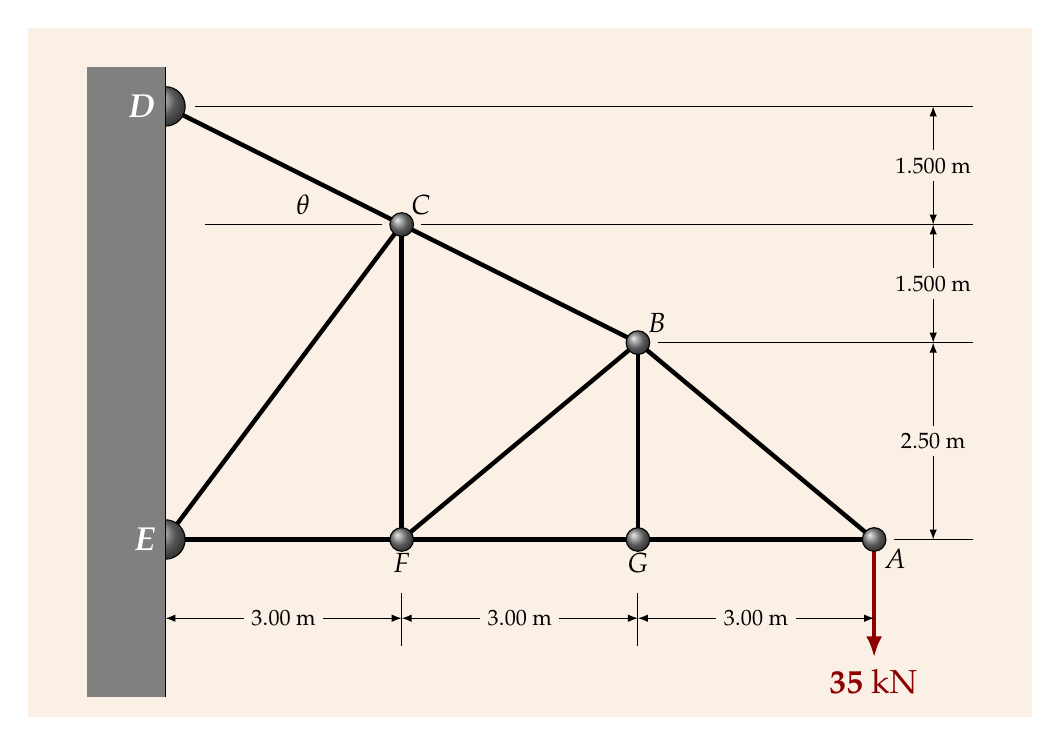
\begin{tikzpicture}[scale=\scale]
	\coordinate (A) at (9,0);
	\coordinate (B) at (6,2.5);
	\coordinate (C) at (3,4);
	\coordinate (D) at (0,5.5);
	\coordinate (E) at (0,0);
	\coordinate (F) at (3,0);
	\coordinate (G) at (6,0);

	\fill[Linen] (-1.75,-2.25) rectangle (11,6.5);

	\draw[ultra thick] (A) -- (B);
	\draw[ultra thick] (B) -- (C);
	\draw[ultra thick] (C) -- (D);
	\draw[ultra thick] (E) -- (F);
	\draw[ultra thick] (F) -- (G);
	\draw[ultra thick] (G) -- (A);
	\draw[ultra thick] (B) -- (G);
	\draw[ultra thick] (C) -- (F);
	\draw[ultra thick] (C) -- (E);
	\draw[ultra thick] (B) -- (F);

		\draw[ultra thick, saitMaroon,arrows={-Latex[scale=0.75]}] (A) -- ++ (0,-1.5) node[below]
	{\large$\bm{\mathrm{ 35 \text { kN} }_{}}$};

	\shadedraw [draw=black, ball color = gray] (A) circle (0.15cm) node[below right] {$A$};
	\shadedraw [draw=black, ball color = gray] (B) circle (0.15cm) node[above right] {$B$};
	\shadedraw [draw=black, ball color = gray] (C) circle (0.15cm) node[above right] {$C$};
	\shadedraw [draw=black, ball color = gray](D) circle (0.25cm);
	\shadedraw [draw=black, ball color = gray] (E) circle (0.25cm);
	\shadedraw [draw=black, ball color = gray] (F) circle (0.15cm) node[below=0.5mm] {$F$};
	\shadedraw [draw=black, ball color = gray] (G) circle (0.15cm) node[below=0.5mm] {$G$};
	\fill[gray] (-1,-2) rectangle (0, 6);
	\draw[black](0,-2) -- (0,6);
	\node[left, white] at (D) {\large $\bm D$};
	\node[left, white] at (E) {\large $\bm E$};

	\node at ($ (C) + (-1.25, 0.25)  $) {\normalsize $\theta$};
	\draw ($ (C)+(-0.25,0)  $) -- ++(-2.25, 0);

	\draw ($ (F)+(0,-0.675)  $) -- ++ (0, -0.675);
	\draw ($ (G)+(0,-0.675)  $) -- ++ (0, -0.675);
	\draw ($ (A)+(0.25,0)  $) -- ++ (1, 0);
	\draw ($ (B)+(0.25,0)  $) -- ++ (4, 0);
	\draw ($ (C)+(0.25,0)  $) -- ++ (7, 0);
	\draw ($ (D)+(0.375,0)  $) -- ++ (9.875, 0);
	\footnotesize
	\draw[arrows={Latex[scale=0.75]-Latex[scale=0.75]}, >=stealth] (9.75,0) -- node[fill=Linen] {$2.50\text{ m}$} (9.75, 2.5);
	\draw[arrows={Latex[scale=0.75]-Latex[scale=0.75]}, >=stealth] (9.75,2.5) -- node[fill=Linen] {$1.500\text{ m}$} (9.75, 4);
	\draw[arrows={Latex[scale=0.75]-Latex[scale=0.75]}, >=stealth] (9.75,4) -- node[fill=Linen] {$1.500\text{ m}$}(9.75, 5.5);
	\draw[arrows={Latex[scale=0.75]-Latex[scale=0.75]}, >=stealth] (0,-1) -- node[fill=Linen] {$3.00\text{ m}$} (3, -1);
	\draw[arrows={Latex[scale=0.75]-Latex[scale=0.75]}, >=stealth] (3,-1) -- node[fill=Linen] {$3.00\text{ m}$}  (6, -1);
	\draw[arrows={Latex[scale=0.75]-Latex[scale=0.75]}, >=stealth] (6,-1) -- node[fill=Linen] {$3.00\text{ m}$}  (9, -1);
\end{tikzpicture}

%   \parb
%   Determine the internal forces in each truss member.
%  \end{myexam}
%
% \end{frame}

%%%%%%%%%%%%%%%%%%%%%%%%%%%%%%%%%%%%%%%%%%%%%%%%%%%%%%%%%%%%%%%%%%%%%%%%%%%%%%%
\scriptsize\raggedright
\begin{frame}

 \def\scale{0.65}

 \begin{textblock*}{0.65\linewidth}(0.5cm, 0.25cm)
  % !TEX root = ../../Beamer/07MoJ/07MoJ.tex

\begin{tikzpicture}[scale=\scale]
	\coordinate (A) at (9,0);
	\coordinate (B) at (6,2.5);
	\coordinate (C) at (3,4);
	\coordinate (D) at (0,5.5);
	\coordinate (E) at (0,0);
	\coordinate (F) at (3,0);
	\coordinate (G) at (6,0);

	\scriptsize

	\uncover<1-6>{
		\pgfoonew \AB=new rrect(A,B,Azure4,Azure2,black,0.25,0.25,0.25,0.125);
	}
	\uncover<7-15>{
		\draw (B)--node[yshift=0.25cm,sloped,Tomato4]{$54.671\,$kN (T)}(A);
		\pgfoonew \AB=new rrect(A,B,Tomato4,Tomato2,black,0.25,0.25,0.25,0.125);
		\draw[-latex, thick] (A)--+(140.2:1.125);
		\draw[-latex, thick] (B)--+(-39.8:1.125);
	}
	\uncover<1-11>{
		\pgfoonew \BC=new rrect(B,C,Azure4,Azure2,black,0.25,0.25,0.25,0.125);
	}
	\uncover<12-15>{
		\draw (C)--node[yshift=0.25cm,sloped,Tomato4]{$58.696\,$kN (T)}(B);
		\pgfoonew \BC=new rrect(B,C,Tomato4,Tomato2,black,0.25,0.25,0.25,0.125);
		\draw[-latex, thick] (C)--+(-26.565:0.875);
		\draw[-latex, thick] (B)--+(153.44:0.875);
	}
	\uncover<1-14>{
		\pgfoonew \CD=new rrect(C,D,Azure4,Azure2,black,0.25,0.25,0.25,0.125);
	}
	\uncover<15>{
		\draw (D)--node[yshift=0.25cm,sloped,Tomato4]{$64.031\,$kN (T)}(C);
		\pgfoonew \CD=new rrect(C,D,Tomato4,Tomato2,black,0.25,0.25,0.25,0.125);
		\draw[-latex, thick] ($(D)+(-26.565:0.125)$) -- +(-26.565:0.875cm);
		\draw[-latex, thick] (C) -- +(153.44:0.875cm);
	}
	\uncover<1-13>{
		\pgfoonew \EF=new rrect(E,F,Azure4,Azure2,black,0.25,0.25,0.25,0.125);
	}
	\uncover<14-15>{
		\draw (E)--node[yshift=-0.25cm,Chartreuse4]{$52.499\,$kN (C)}(F);
		\pgfoonew \EF=new rrect(E,F,Chartreuse4,Chartreuse2,black,0.25,0.25,0.25,0.125);
		\draw[latex-, thick] ($(E)+(0.25,0)$)--+(0:0.875);
		\draw[latex-, thick] ($(F)+(-0.125,0)$)--+(180:0.875);
	}
	\uncover<1-9>{
		\pgfoonew \FG=new rrect(F,G,Azure4,Azure2,black,0.25,0.25,0.25,0.125);
	}
	\uncover<10-15>{
		\draw (F)--node[yshift=-0.25cm,Chartreuse4]{$41.999\,$kN (C)}(G);
		\pgfoonew \FG=new rrect(F,G,Chartreuse4,Chartreuse2,black,0.25,0.25,0.25,0.125);
		\draw[latex-, thick] ($(G)+(-0.125,0)$)--+(180:0.875);
		\draw[latex-, thick] ($(F)+(0.125,0)$)--+(0:0.875);
	}
	\uncover<1-7>{
		\pgfoonew \GA=new rrect(G,A,Azure4,Azure2,black,0.25,0.25,0.25,0.125);
	}
	\uncover<8-15>{
		\draw (G)--node[yshift=-0.25cm,Chartreuse4]{$41.999\,$kN (C)}(A);
		\pgfoonew \GA=new rrect(G,A,Chartreuse4,Chartreuse2,black,0.25,0.25,0.25,0.125);
		\draw[latex-, thick] (A)--+(180:0.875);
		\draw[latex-, thick] (G)--+(0:0.875);
	}
	\uncover<1-3>{
		\pgfoonew \BG=new rrect(B,G,Azure4,Azure2,black,0.25,0.25,0.25,0.125);
	}
	\uncover<4-15>{
		\node[xshift=-0.2125cm] at ($(G)!.5!(B)$){$0$};
		\begin{scope}[opacity=0.35]
			\pgfoonew \BG=new rrect(B,G,Azure4,white,black,0.25,0.25,0.25,0.125);
		\end{scope}
	}
	\uncover<1-12>{
		\pgfoonew \CF=new rrect(C,F,Azure4,Azure2,black,0.25,0.25,0.25,0.125);
	}
	\uncover<13-15>{
		\draw (F)--node[xshift=-2mm,yshift=0.25cm,sloped,Tomato4]{$8.7501\,$kN (T)}(C);
		\pgfoonew \CF=new rrect(C,F,Tomato4,Tomato2,black,0.25,0.25,0.25,0.125);
		\draw[-latex, thick] (F) -- +(90:0.875cm);
		\draw[-latex, thick] (C) -- +(270:0.875cm);
	}
	\uncover<1-14>{
	\pgfoonew \CE=new rrect(C,E,Azure4,Azure2,black,0.25,0.25,0.25,0.125);
	}
	\uncover<15>{
	\draw (E)--node[yshift=0.25cm,Chartreuse4,sloped]{$7.9542\,$kN (C)}(C);
	\pgfoonew \CE=new rrect(C,E,Chartreuse4,Chartreuse2,black,0.25,0.25,0.25,0.125);
	\draw[latex-, thick] ($(E)+(53.13:0.25)$)--+(53.13:0.875);
	\draw[latex-, thick] (C)--+(233.13:0.875);
	}
	\uncover<1-11>{
		\pgfoonew \BF=new rrect(B,F,Azure4,Azure2,black,0.25,0.25,0.25,0.125);
	}
	\uncover<12->{
		\draw (F)--node[yshift=0.25cm,sloped,Chartreuse4]{$13.668\,$kN (C)}(B);
		\pgfoonew \BF=new rrect(B,F,Chartreuse4,Chartreuse2,black,0.25,0.25,0.25,0.125);
		\draw[latex-, thick] (B)--+(219.8:0.875);
		\draw[latex-, thick] (F)--+(39.806:0.875);
	}


	\draw[ultra thick, saitMaroon, -Latex] (A) -- ++ (0,-1.5) node[below]
	{\normalsize$\bm{\mathrm{ 35\,\text{kN}}$}};



	\uncover<1-3>{
		\draw ($ (F)+(0,-0.625)  $) -- ++ (0, -0.5);
		\draw ($ (G)+(0,-0.625)  $) -- ++ (0, -0.5);
		\draw ($ (A)+(0.25,0)  $) -- ++ (1, 0);
		\draw ($ (B)+(0.375,0)  $) -- ++ (3.875, 0);
		\draw ($ (C)+(0.5,0)  $) -- ++ (6.75, 0);
		\draw ($ (D)+(0.5,0)  $) -- ++ (9.85, 0);

		\draw[latex-latex] (9.75,0) -- node[fill=white] {$2.50\text{ m}$} (9.75, 2.5);
		\draw[latex-latex] (9.75,2.5) -- node[fill=white] {$1.50\text{ m}$} (9.75, 4);
		\draw[latex-latex] (9.75,4) -- node[fill=white] {$1.500\text{ m}$}(9.75, 5.5);
		\draw[latex-latex] (0,-0.875) -- node[fill=white] {$3.00\text{ m}$} (3, -0.875);
		\draw[latex-latex] (3,-0.875) -- node[fill=white] {$3.00\text{ m}$}  (6, -0.875);
		\draw[latex-latex] (6,-0.875) -- node[fill=white] {$3.00\text{ m}$}  (9, -0.875);

	}

	\uncover<1->{
		\draw ($ (C)+(-0.5,0)  $) -- ++(-2, 0);
	}

	\uncover<1>{
		\node at ($ (C) + (-1.75, 0.325)  $) {\normalsize $\theta$};
	}



	\uncover<1->{
		\draw[latex-latex] ($(A)+(-2,0)$)arc(180:140.2:2)node[midway, fill=white, inner sep=0.25mm]{$39.806\degree$};
	}
	\uncover<2->{
		\draw[latex-latex]($ (C)+(-2.25,0) $)  arc (180:153:2.25) node[xshift=-0.0625cm, midway, fill=white, inner sep = 0.2mm] {$26.565\degree$};
	}
	\uncover<3->{
		\draw[arrows={Latex[scale=0.75]-Latex[scale=0.75]}] ($ (E)+(1.75,0) $)  arc (0:53.13:1.75cm) node[fill=white, inner sep = 0.125em] at ($ (E)+(23:1.85) $) {$53.130\degree$};
	}


	\shadedraw [draw=black, ball color = gray] (A) circle (0.075cm) node[below right] {\small $A$};
	\shadedraw [draw=black, ball color = gray] (B) circle (0.075cm) node[above right] {\small $B$};
	\shadedraw [draw=black, ball color = gray] (C) circle (0.075cm) node[above right] {\small $C$};
	\shadedraw [draw=black, ball color = gray] (D) circle (0.25cm);
	\shadedraw [draw=black, ball color = gray] (E) circle (0.25cm);
	\shadedraw [draw=black, ball color = gray] (F) circle (0.075cm) node[below=0.5mm] {\small $F$};
	\shadedraw [draw=black, ball color = gray] (G) circle (0.075cm) node[below=0.5mm] {\small $G$};
	\fill[gray] (-1,-2) rectangle (0, 6);
	\draw[black](0,-2) -- (0,6);
	\node[left, white] at (D) {\normalsize $\bm D$};
	\node[left, white] at (E) {\normalsize $\bm E$};




\end{tikzpicture}

 \end{textblock*}

 \only<1-6>{
  \begin{textblock*}{3.75cm}(8.5cm,0.25cm)

   \begin{mybox}[title=Calculate Angles, colback=Linen]
    \scriptsize
    \begin{align*}
     \uncover<1-6>{
     \angle BAG & = \tan^{-1} \left[\frac{2.50}{3.00}\right]  \\
                & = 39.806\degree                             \\\\
     }
     \uncover<2-6>{
     \theta     & = \tan^{-1} \left[\frac{1.500}{3.00}\right] \\
                & = 26.565\degree                             \\\\
     }
     \uncover<3-6>{
     \angle CEF & = \tan^{-1} \left[\frac{4.00}{3.00}\right]  \\
                & = 53.130\degree
     }
    \end{align*}

    \vspace{-1.25em}
   \end{mybox}
  \end{textblock*}
 }


 \begin{textblock*}{8cm}(2.5cm, 5.5cm)
  \uncover<4-6>{
   \begin{mybox}[left=0.25cm, right=0.25cm, title=Notice:, colback=Linen]
    \parm
    \begin{enumerate}
     \item By inspection, truss member $BG$ is a \textcolor{saitMaroon}{\bfseries zero-force} member.\parm
     \item <5-6> We can start at joint $A$ and proceed through the truss joints $A\rightarrow G\rightarrow B\rightarrow C\rightarrow F$, without calculating the reactions at $D$ and $E$.\parm
     \item <6> Finding the reactions at $D$ and $E$ {\bfseries is} useful to verify our results; if we have not made mistakes, then the sum of all forces acting at $D$ (including the reaction) will equal $0$. Similarly, the sum of all forces acting at $E$ will equal $0$.
    \end{enumerate}
   \end{mybox}
  }
 \end{textblock*}


 \only<7-9>{
  \begin{textblock*}{3.75cm}(8.5cm,0.25cm)
   \begin{mybox}[left=0.25cm, right=0.25cm, title=Free Body Diagram: $\bm A$, colback=Linen]
    \begin{center}
     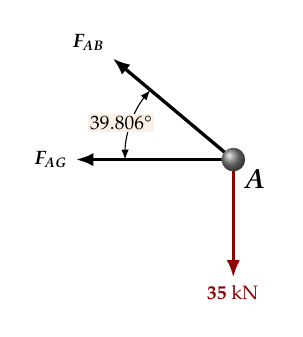
\begin{tikzpicture}[scale=\scale]
  \scriptsize
  \coordinate (A) at (0,0);
  \draw[very thick,arrows={-Latex[scale=0.75]}] (A) -- (140:2cm) node[above left] {$\bm{F_{AB}}$};
  \draw[very thick,arrows={-Latex[scale=0.75]}] (A) -- (180:2cm) node[left] {$\bm{F_{AG}}$};
  \draw[very thick, saitMaroon,arrows={-Latex[scale=0.75]}] (A) -- ++ (0,-1.5) node[below]
  {$\bm{\mathrm{ 35 \text { kN} }_{}}$};

  \draw[arrows={Latex[scale=0.75]-Latex[scale=0.75]}] ($ (A)+(-1.375,0) $)  arc (180:140.2:1.375cm) node[fill=Linen, inner sep = 0.125em] at ($ (A)+(162:1.5) $) {\scriptsize $39.806\degree$};
  \normalsize
  \shade [ball color = gray] (A) circle (0.15cm) node[below right] {$\bm A$};
\end{tikzpicture}

    \end{center}
   \end{mybox}
  \end{textblock*}

  \begin{textblock*}{8cm}(2.5cm, 5.5cm)
   \uncover<7-9>{
    \begin{mybox}[left=0.25cm, right=0.25cm, title=Joint $\bm A$, colback=Linen]
     \scriptsize\raggedright
     \uncover<7-9>{
      Sum the $y$ components first, so that we have only one variable and don't need to solve a system of simultaneous equations:
     }
     \begin{align*}
      \uncover<8-9>{
      \Sigma F_y         & = F_{AB}\sin 39.806\degree - 35\text{ kN} = 0 \\
      \Rightarrow F_{AB} & = 54.671\text{ kN}                            \\\\
      }
      \uncover<9>{
      \Sigma F_x         & = -F_{AB}\cos 39.806\degree - F_{AG} = 0      \\
      \Rightarrow F_{AG} & = -54.671\cos 39.806\degree\text{ kN}         \\
                         & = -41.999 \text{ kN}
      }
     \end{align*}
    \end{mybox}
   }
  \end{textblock*}
 }

 \only<10-11>{
  \begin{textblock*}{3.75cm}(8.5cm,0.25cm)
   \begin{mybox}[left=0.25cm, right=0.25cm, title=Free Body Diagram: $\bm G$, colback=Linen]
    \scriptsize\raggedright
    % $G$ is a trivial joint.
    \begin{center}
     \input{../../pikz/07MoJ/07truss03SolnJointGLinen.tex}
    \end{center}
   \end{mybox}
  \end{textblock*}

  \begin{textblock*}{8cm}(2.5cm, 5.5cm)
   \uncover<10-12>{
    \begin{mybox}[left=0.25cm, right=0.25cm, title=Joint $\bm G$, colback=Linen]
     \scriptsize\raggedright

     \textcolor{saitMaroon}{\bfseries Known} forces, such as $F_{AG}$, are drawn in their actual direction.\pars \textcolor{saitMaroon}{\bfseries Unknown} forces, such as $F_{FG}$ and $F_{BG}$, are drawn in tension with the arrowheads pointing away from the joint.
		 \uncover<11-12>{
     \begin{align*}
      \Sigma F_x         & = -F_{FG}-41.999\text{ kN} = 0 \\
      \Rightarrow F_{FG} & = -41.999\text{ kN}
			\end{align*}
      }
     \uncover<12>{%
      Trivial joints, such as $G$, can be solved without drawing an $FBD$ or performing the algebra, if desired.
     }
    \end{mybox}
   }
  \end{textblock*}
 }

 \only<13-18>{
  \begin{textblock*}{4.25cm}(8.25cm,0.25cm)
   \begin{mybox}[left=0.25cm, right=0.25cm, title=Free Body Diagram: $\bm B$, colback=Linen]
    \begin{center}
     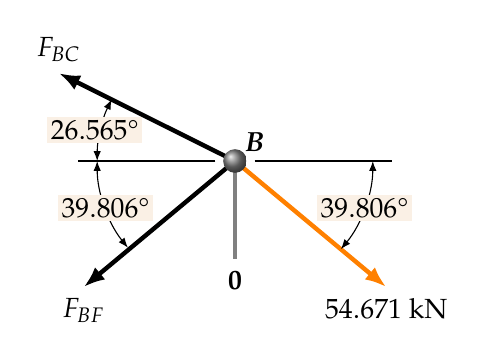
\begin{tikzpicture}[scale=\scale]

  \coordinate (B) at (0,0);
  % \footnotesize
  \draw[ultra thick, arrows={-Latex[scale=0.75]}, orange] (B) -- (-39.806:2.5cm) node[black, below] {$54.671\text{ kN}$};
  \draw[ultra thick, arrows={-Latex[scale=0.75]}] (B) -- (153.5:2.5cm) node[above] {$F_{BC}$};
  \draw[ultra thick, arrows={-Latex[scale=0.75]}] (B) -- (219.8:2.5cm) node[below] {$F_{BF}$};

  \draw[ultra thick, gray] (B) -- ++(-90:1.25cm) node[below, black]  {$\bm 0$};
  \shade [ball color = gray] (B) circle (0.15cm) node[above right] {$\bm B$};
  \draw ($ (B)+(0.25, 0) $) -- +(1.75, 0);
  \draw ($ (B)-(0.25, 0) $) -- +(-1.75, 0);

  % \footnotesize
  \draw[arrows={Latex[scale=0.75]-Latex[scale=0.75]}] ($ (B)+(-1.75,0) $)  arc (180:219:1.75cm) node[fill=Linen, inner sep = 0.125em] at ($ (B)+(200:1.75) $) {$39.806\degree$};
  \draw[arrows={Latex[scale=0.75]-Latex[scale=0.75]}] ($ (B)+(1.75,0) $)  arc (0:-39.8:1.75cm) node[fill=Linen, inner sep = 0.125em] at ($ (B)+(-20:1.75) $) {$39.806\degree$};
  \draw[arrows={Latex[scale=0.75]-Latex[scale=0.75]}] ($ (B)+(-1.75,0) $)  arc (180:153.5:1.75cm) node[fill=Linen, inner sep = 0.125em] at ($ (B)+(167.5:1.825) $) {$26.565\degree$};

\end{tikzpicture}

    \end{center}
   \end{mybox}
  \end{textblock*}
 }

 \begin{textblock*}{9cm}(2cm, 5.5cm)
  \uncover<13-14>{
   \begin{mybox}[left=0.25cm, right=0.25cm, title=Joint $\bm B$, colback=Linen]
    \vspace{-0.25cm}
    \begin{align*}			%
     \Sigma F_y   = & \quad F_{BC}\sin 26.565\degree - F_{BF}\sin 39.806\degree -54.671\sin 39.806\degree \text{ kN}  = 0                  \\
     \Rightarrow    & \quad F_{BC}\sin 26.565\degree - F_{BF}\sin 39.806\degree                                         = 35.000\text{ kN} \\\\
     \Sigma F_x   = & \quad 54.671\cos 39.806\degree-F_{BC}\cos 26.565\degree -F_{BF}\cos 39.806\degree = 0                                \\
     \Rightarrow    & \quad F_{BC}\cos 26.565\degree +F_{BF}\cos 39.806\degree = 41.999\text{ kN}
    \end{align*}

    \uncover<14>{
     Use the \textcolor{saitMaroon}{\bfseries system-solver} on your calculator to find $ F_{BC}=58.696\text{ kN},\;F_{BF}=-13.668\text{ kN}  $
    }
   \end{mybox}
  }
 \end{textblock*}

 \only<19-21>{
  \begin{textblock*}{4.25cm}(8.25cm,0.25cm)
   \begin{mybox}[left=0.25cm, right=0.25cm, title=Free Body Diagram, colback=Linen]
    \begin{center}
     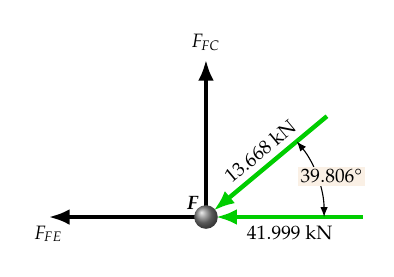
\begin{tikzpicture}[scale=\scale]

	\coordinate (F) at (0,0);
	\scriptsize
	\draw[ultra thick, {Latex[scale=0.75]-}, Green3] ($ (F)+(39.8:0.125cm) $) -- node[black, above, sloped] {$13.668\text{ kN}$}(39.806:2cm) ;
	\draw[ultra thick, {Latex[scale=0.75]-}, Green3] ($ (F)+(0:0.125cm) $) -- node[black, below] {$41.999\text{ kN}$}(0:2cm) ;
	\draw[ultra thick, {-Latex[scale=0.75]}] (F) -- (90:2cm) node[above] {$F_{FC}$};
	\draw[ultra thick, {-Latex[scale=0.75]}] (F) -- (180:2cm) node[below] {$F_{FE}$};

	\shade [ball color = gray] (F) circle (0.15cm) node[above left] {$\bm F$};
	\draw[arrows={Latex[scale=0.75]-Latex[scale=0.75]}] ($ (F)+(1.5,0) $)  arc (0:39.8:1.5cm) node[fill=Linen, inner sep = 0.125em] at ($ (F)+(18:1.675) $) {$39.806\degree$};

\end{tikzpicture}

    \end{center}
   \end{mybox}
  \end{textblock*}


  \begin{textblock*}{9cm}(2cm, 5.5cm)
   \uncover<20->{
    \begin{mybox}[left=0.25cm, right=0.25cm, title=Joint F, colback=Linen]
     \begin{align*}
      \Sigma F_x         & = -F_{FE} -13.668\cos 39.806\degree \text{kN} - 41.999\,\text{kN}  = 0 \\
      \Rightarrow F_{FE} & = -52.499\,\text{kN}                                                   \\\\
      \uncover<21->{
      \Sigma F_y         & = F_{FC}-13.668\sin 39.806^\circ = 0                                   \\
      \Rightarrow F_{FC} & = 8.7501\,\text{kN}
      }
     \end{align*}
    \end{mybox}
   }
  \end{textblock*}
 }

 \only<22->{
  \begin{textblock*}{4.25cm}(8.25cm,0.25cm)
   \def\scale{0.75}
   \begin{mybox}[left=0.25cm, right=0.25cm, title=Free Body Diagram, colback=Linen]
    \begin{center}
     % !TEX root = ../../Beamer/04MoJ/04MoJSxS.tex

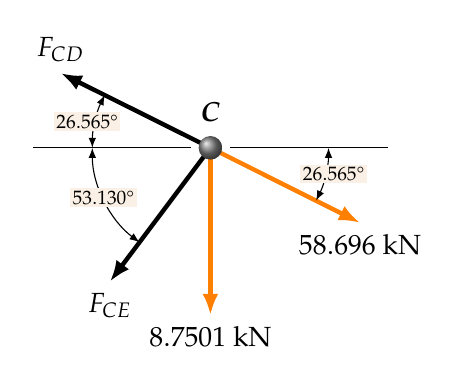
\begin{tikzpicture}[scale=\scale]

  \coordinate (C) at (0,0);
  % \footnotesize
  \draw[ultra thick, {-Latex[scale=0.75]}, orange] ($ (C)+(-26.6:0.125cm) $) -- (-26.6:2.125cm) node[black, below] {$58.696\text{ kN}$};
  \draw[ultra thick, {-Latex[scale=0.75]}, orange] ($ (C)+(270:0.125cm) $) -- (270:2.125cm) node[black, below] {$8.7501\text{ kN}$};
  \draw[ultra thick, {-Latex[scale=0.75]}] ($ (C)+(153.5:0.125cm) $) -- (153.5:2.125cm) node[black, above] {$F_{CD}$};
  \draw[ultra thick, {-Latex[scale=0.75]}] ($ (C)+(233.1:0.125cm) $) -- (233.1:2.125cm) node[black, below] {$F_{CE}$};

  \draw ($ (C)+(0.25, 0) $) -- +(2,0);
  \draw ($ (C)+(-0.25, 0) $) -- +(-2,0);

  \shade [ball color = gray] (C) circle (0.15cm) node[above=.2cm] {$\bm C$};

  \scriptsize
  \draw[arrows={Latex[scale=0.75]-Latex[scale=0.75]}] ($ (C)+(1.5,0) $)  arc (0:-26.565:1.5cm) node[fill=Linen, inner sep = 0.125em] at ($ (C)+(-12:1.6) $) {$26.565\degree$};
  \draw[arrows={Latex[scale=0.75]-Latex[scale=0.75]}] ($ (C)-(1.5,0) $)  arc (180:153.5:1.5cm) node[fill=Linen, inner sep = 0.125em] at ($ (C)+(168:1.6) $) {$26.565\degree$};
  \draw[arrows={Latex[scale=0.75]-Latex[scale=0.75]}] ($ (C)-(1.5,0) $)  arc (180:233.1:1.5cm) node[fill=Linen, inner sep = 0.125em] at ($ (C)+(205:1.5) $) {$53.130\degree$};

\end{tikzpicture}

    \end{center}
   \end{mybox}
  \end{textblock*}

%   \begin{textblock*}{9cm}(2cm, 5.5cm)
%    \uncover<23-24>{
%     \begin{mybox}[left=0.25cm, right=0.25cm, title=Joint C, colback=Linen]
%      \begin{align*}
%       \Sigma F_x            = -F_{CD}\cos 26.565\degree - F_{CE}\cos 53.130\degree + 58.696\cos 26.565\degree     & = 0       \\
%       \Rightarrow F_{CD}\cos 26.565\degree + F_{CE}\cos 53.130\degree                                             & = 52.499  \\\\
%       \Sigma F_y            = F_{CD}\sin 26.565\degree -F_{CE}\sin 53.130\degree -8.7501-58.696\sin 26.565\degree & = 0       \\
%       \Rightarrow   F_{CD}\sin 26.565\degree -F_{CE}\sin 53.130\degree                                            & =  34.999
%      \end{align*}
%      \parm
%      \uncover<24>{
%       \centering
%       From your calculator: $F_{CD}=64.031\text{ kN},\;F_{CE}=-7.9542\text{ kN}$
%      }

%     \end{mybox}
%    }
%   \end{textblock*}
%  }
% \end{frame}

% %%%%%%%%%%%%%%%%%%%%%%%%%%%%%%%%%%%%%%%%%%%%%%%%%%%%%%%%%%%%%%%%%%%%%%%%%%%%%%%%


\begin{frame}

 \def\scale{0.65}

 \begin{textblock*}{0.65\linewidth}(0.375cm, 0cm)
  
% !TEX root = ../../Beamer/04MoJ/04MoJSxS.tex

\begin{tikzpicture}[scale=\scale]
	\coordinate (A) at (9,0);
	\coordinate (B) at (6,2.5);
	\coordinate (C) at (3,4);
	\coordinate (D) at (0,5.5);
	\coordinate (E) at (0,0);
	\coordinate (F) at (3,0);
	\coordinate (G) at (6,0);

	\fill[white] (-1.75,-2.25) rectangle (11,6.5);

	\draw[ultra thick, saitMaroon,arrows={-Latex[scale=0.75]}] (A) -- ++ (0,-1.5) node[below]
	{$\normalsize\bm{\mathrm{ 35 \text { kN} }_{}}$};

	\only<1>{
		\draw[ultra thick] (A) -- (B);
		\draw[ultra thick] (B) -- (C);
		\draw[ultra thick] (C) -- (D);
		\draw[ultra thick] (E) -- (F);
		\draw[ultra thick] (F) -- (G);
		\draw[ultra thick] (G) -- (A);
		\draw[ultra thick] (B) -- (G);
		\draw[ultra thick] (C) -- (F);
		\draw[ultra thick] (C) -- (E);
		\draw[ultra thick] (B) -- (F);

		\shade [draw=black, ball color = gray] (A) circle (0.15cm) node[below right] {$A$};
		\shade [draw=black, ball color = gray] (B) circle (0.15cm) node[above right] {$B$};
		\shade [draw=black, ball color = gray] (C) circle (0.15cm) node[above right] {$C$};
		\shade [draw=black, ball color = gray](D) circle (0.25cm);
		\shade [draw=black, ball color = gray] (E) circle (0.25cm);
		\shade [draw=black, ball color = gray] (F) circle (0.15cm) node[below=0.5mm] {$F$};
		\shade [draw=black, ball color = gray] (G) circle (0.15cm) node[below=0.5mm] {$G$};
		\fill[gray] (-1,-2) rectangle (0, 6);
		\draw[black](0,-2) -- (0,6);
	}

	\only<2->{
		\draw[ultra thick, llHeaderGrey] (A) -- (B);
		\draw[ultra thick, llHeaderGrey] (B) -- (C);
		\draw[ultra thick, llHeaderGrey] (C) -- (D);
		\draw[ultra thick, llHeaderGrey] (E) -- (F);
		\draw[ultra thick, llHeaderGrey] (F) -- (G);
		\draw[ultra thick, llHeaderGrey] (G) -- (A);
		\draw[ultra thick, llHeaderGrey] (B) -- (G);
		\draw[ultra thick, llHeaderGrey] (C) -- (F);
		\draw[ultra thick, llHeaderGrey] (C) -- (E);
		\draw[ultra thick, llHeaderGrey] (B) -- (F);

		\fill [llHeaderGrey] (A) circle (0.15cm) node[below right] {$A$};
		\fill [llHeaderGrey] (B) circle (0.15cm) node[above right] {$B$};
		\fill [llHeaderGrey] (C) circle (0.15cm) node[above right] {$C$};
		\fill [llHeaderGrey](D) circle (0.25cm);
		\fill [llHeaderGrey] (E) circle (0.25cm);
		\fill [llHeaderGrey] (F) circle (0.15cm) node[below=0.5mm] {$F$};
		\fill [llHeaderGrey] (G) circle (0.15cm) node[below=0.5mm] {$G$};
		\fill[llHeaderGrey] (-1,-2) rectangle (0, 6);
		\draw[gray](0,-2) -- (0,6);
	}





	\node[below left, white] at (D) {\normalsize $\bm D$};
	\node[left, white] at (E) {\normalsize $\bm E$};



	\draw[arrows={Latex[scale=0.75]-Latex[scale=0.75]}] ($ (C)+(-1.85,0) $)  arc (180:153:1.85cm) node[fill=white, inner sep = 0.2mm, outer sep=0mm] at ($ (C)+(167:1.9) $) {$26.565\degree$};
	\draw ($ (C)+(-0.25,0)  $) -- ++(-2.25, 0);

	\draw ($ (F)+(0,-0.675)  $) -- ++ (0, -0.675);
	\draw ($ (G)+(0,-0.675)  $) -- ++ (0, -0.675);
	\draw ($ (A)+(0.25,0)  $) -- ++ (1, 0);
	\draw ($ (B)+(0.25,0)  $) -- ++ (4, 0);
	\draw ($ (C)+(0.25,0)  $) -- ++ (7, 0);
	\draw ($ (D)+(0.375,0)  $) -- ++ (9.875, 0);
	\footnotesize
	\draw[arrows={Latex[scale=0.75]-Latex[scale=0.75]}] (9.75,0) -- node[fill=white] {$2.50\text{ m}$} (9.75, 2.5);
	\draw[arrows={Latex[scale=0.75]-Latex[scale=0.75]}] (9.75,2.5) -- node[fill=white] {$1.500\text{ m}$} (9.75, 4);
	\draw[arrows={Latex[scale=0.75]-Latex[scale=0.75]}] (9.75,4) -- node[fill=white] {$1.500\text{ m}$}(9.75, 5.5);
	\draw[arrows={Latex[scale=0.75]-Latex[scale=0.75]}] (0,-1) -- node[fill=white] {$3.00\text{ m}$} (3, -1);
	\draw[arrows={Latex[scale=0.75]-Latex[scale=0.75]}] (3,-1) -- node[fill=white] {$3.00\text{ m}$}  (6, -1);
	\draw[arrows={Latex[scale=0.75]-Latex[scale=0.75]}] (6,-1) -- node[fill=white] {$3.00\text{ m}$}  (9, -1);

	\only<2->{
		\draw [ultra thick, saitMaroon, line cap = round, arrows={-Latex[scale=0.75]}] (E) -- (1.25,0) node[above]{$\bm{E_{x}}$};
		\draw [ultra thick, saitMaroon, line cap = round, arrows={-Latex[scale=0.75]}] (E) -- (0,1.25) node[right]{$\bm{E_{y}}$};
	}
	\only<3->{
		\draw [ultra thick, saitMaroon, line cap = round, arrows={-Latex[scale=0.75]}] (D) -- +(153.4:1.25) node[below]{$\bm{R_D}$};
	}
\end{tikzpicture}

 \end{textblock*}

 \begin{textblock*}{3.5cm}(8.5cm,0.25cm)

  \begin{mybox}[title=Finished\ldots, colback=Linen]
   \scriptsize
   \begin{align*}
    AB & = 54.7\text{ kN (T)}  \\
    AG & = 42.0\text{ kN (C)}  \\
    BC & = 58.7\text{ kN (T)}  \\
    BF & = 13.69\text{ kN (C)} \\
    BG & = 0                   \\
    CD & = 64.0\text{ kN (T)}  \\
    CE & = 7.95\text{ kN (C)}  \\
    CF & = 8.75\text{ kN (T)}  \\
    EF & = 52.5\text{ kN (C)}
   \end{align*}
   \centering
   But are they correct?
  \end{mybox}
 \end{textblock*}

 \begin{textblock*}{5cm}(1cm, 5.75cm)
  \uncover<2-4>{
   \begin{mybox}[left=0.25cm, right=0.25cm, title=Check The Results!, colback=Linen]
    Consider only the external forces acting on the truss:
    \begin{enumerate}
     \item<2->  There is a reaction at the pinned connection at $E$,
     \item<3-> There is a connection at $D$ with known direction ($CD$ is a two-force member so the reaction at $D$ has the same line of action as $CD$.)
     \item<4-> There is a $35\text{ kN}$ load at $A$.
    \end{enumerate}
   \end{mybox}
  }
 \end{textblock*}

 \begin{textblock*}{5.75cm}(1cm, 5.75cm)
  \uncover<5-6>{
   \begin{mybox}[left=0.25cm, right=0.25cm, colback=Linen]
    \vspace{-1em}
    \begin{align*}
     \Sigma M_E       & = R_D\cos\,26.565\degree\times 5.50\text{ m} -35\text{ kN}\times 9.00\text{ m}= 0 \\
     \Rightarrow  R_D & = 64.033\text{ kN}
    \end{align*}
    \mini[0.85]{
     \raggedright
     $R_D=64.033\text{ kN}$ which makes it equal (apart from a rounding error) and opposite to $F_{CD}$, the tensile force in $CD$ so $\Sigma F_D=0$.
    }
    \textcolor{green}{\Huge\checkmark}
   \end{mybox}
  }
 \end{textblock*}

 \begin{textblock*}{4.5cm}(7.5cm, 5.75cm)
  \uncover<6-7>{
   \begin{mybox}[left=0.25cm, right=0.25cm, colback=Linen]
    \vspace{-1em}
    \begin{align*}
     \Sigma F_x       & = E_x - R_D\cos\,26.565\degree= 0            \\
     \Rightarrow  E_x & = 57.273\text{ kN}                           \\\\
     \Sigma F_y       & = E_y+R_D\sin 26.565\degree-35\text{ kN} = 0 \\
     \Rightarrow  E_y & = 6.3636\text{ kN}
    \end{align*}
   \end{mybox}
  }
 \end{textblock*}

 \begin{textblock*}{4.25cm}(1cm,5.75cm)
  \uncover<7->{
   \def\scale{0.65}
   \begin{mybox}[left=0.25cm, right=0.25cm, title=Free Body Diagram, colback=Linen]
    \begin{center}
     \input{../../pikz/07MoJ/07truss03SolnJointEReactions.tex}
    \end{center}
   \end{mybox}

  }
 \end{textblock*}

 \begin{textblock*}{6cm}(6cm, 5.75cm)
  \uncover<8>{
   \begin{mybox}[left=0.25cm, right=0.25cm, title=Joint E, colback=Linen]
    \vspace{-1em}
    \begin{align*}
     \Sigma F_x & = 57.273\text{ kN} - 52.499\text{ kN} - 7.9542\cos 39.806\degree \text{kN} \\
                & = 0.00147\text{ kN}\approx 0\quad\textcolor{green}{\checkmark} \\
     \Sigma F_y & = 6.3636\text{ kN}-7.9542\sin 53.130\degree \text{ kN}                     \\
                & =0.000249\text{ kN}\approx 0\quad\textcolor{green}{\checkmark}
    \end{align*}
   \end{mybox}
  }
 \end{textblock*}
\end{frame}




\end{document}
